% <- main.tex
\subsubsection{概要}

2次元平面内でのひも状細胞の挙動の理解のために,この対象をモデル化して,
N個の質点がそれぞれバネで1次元的に繋がれているような状況を考える(図\ref{fig:model})。

\begin{figure}[H]
  \begin{center}
    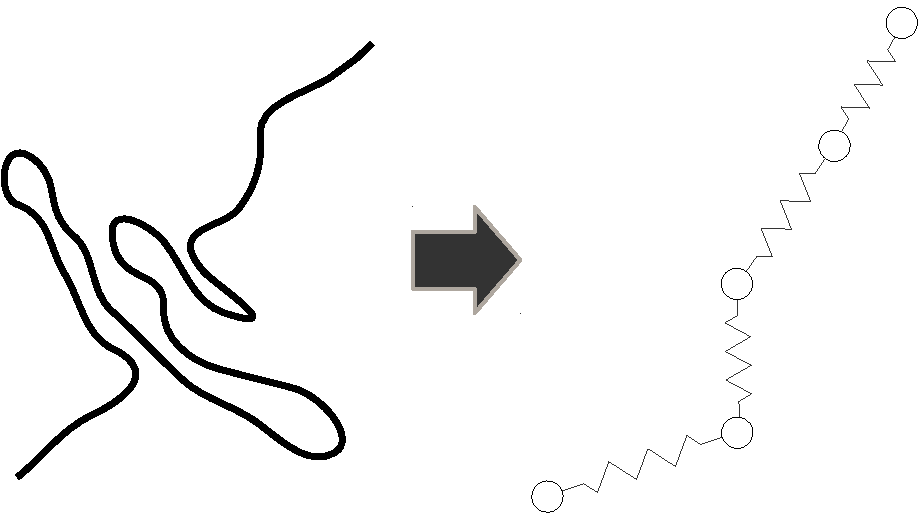
\includegraphics[width=0.5\textwidth]{../img/model.pdf}
    \caption{ひも状細胞の質点とばねによるモデル化}
    \label{fig:model}
  \end{center}
\end{figure}

このとき,これらの質点間に働く力は,バネの伸びによるフック則に従う力$F^{s}$と,
近接点との位置関係によって生じる曲げ弾性による力$F^{b}$である.
また,これらの力の他に,速度に比例する力として粘性抵抗(粘性係数$\gamma$)による力が働くとする。

ひも状細胞の成長を再現するために,各ばねの自然長が一定ではなく,時間の関数として増大していくとし,
これがある閾値を超えた時にそのばねの間に新たに一つ質点を追加することによって
成長過程を記述することにする。

\subsubsection{各質点に対する運動方程式}

$i$番目($i \in [0, N-1]$)の質点に関する運動方程式は,以下のように表される。
\begin{align*}
  m\ddot{\vec{x}}_{i} &= F_{i}^{s} + F_{i}^{b} - \gamma \dot{\vec{x}}_{i}
  \tag{1}\label{e1} \\
  \\
  F_{i}^{s} &= - k_{i-1}(d_{i-1} - n_{i-1}) + k_{i}(d_{i} - n_{i}) 
  \tag{1.a}\label{e1a} \\
  F_{i}^{b} &= E_i\left(\frac{\vec{x}_{i-1} + \vec{x}_{i+1}}{2} - \vec{x}_{i}\right) \\
  &\quad  - \frac{1}{2} E_{i-1}\left(\frac{\vec{x}_{i-2} + \vec{x}_{i+2}}{2} - \vec{x}_{i-1}\right) \\
  &\quad - \frac{1}{2}E_{i+1}\left(\frac{\vec{x}_{i} + \vec{x}_{i+2}}{2} - \vec{x}_{i+1}\right)
  \tag{1.b}\label{e1b}
\end{align*}

\begin{align*}
  \vec{x}_{i} &: i\text{番目の質点の位置ベクトル} \\
  k_{i} &: i\text{番目と}i+1\text{番目の質点間のバネのバネ定数} \\
  n_{i} &: i\text{番目と}i+1\text{番目の質点間のバネの自然長} \\
  d_{i} &: i\text{番目と}i+1\text{番目の質点間の距離} \\
  E_{i} &: i-1,i,i+1\text{番目の3つの質点により決まる曲げ弾性係数}
\end{align*}

ここで,ひもの先端と終端がつながっている場合(これを\textbf{閉な場合}と呼ぶことにする)には
$k_{-1}$や$n_{-1}$,$d_{-1}$,$E_{0}$,$E_{N}$などはラベル$0$の質点とラベル$N-1$の質点の間でそれぞれ定義されるものである.
一方で,ひもの先端と終端が繋がれていない場合(これを\textbf{開な場合}と呼ぶことにする)には,これらの値は定義されず,
$k_{-1} = E_{0} = E_{N-1} = 0$と再定義することにする.

\begin{figure}[H]
  \begin{center}
    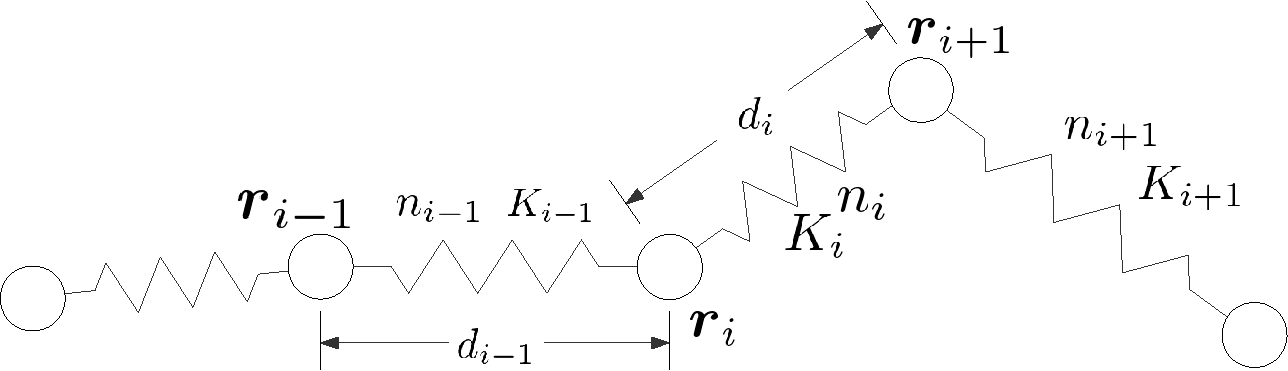
\includegraphics[width=0.7\textwidth]{../img/coordinates.pdf}
    \vspace{0.5cm}
    \caption{質点とばねに関する物理量}
    \label{fig:coodinates}
  \end{center}
\end{figure}


シミュレーションでは実際にこの運動方程式を4次のルンゲクッタ法もしくはオイラー法で計算することによって時間発展を逐次計算していく.

ただ,それぞれの質点要素に関して同時に計算を行うことができるので,力の項の計算を
行列として計算するほうが効率的である。

したがって,これから式(\ref{e1}), (\ref{e1a}), (\ref{e1b})を行列による表記に書き直す。
$x$座標に関する配列を$\vector{x}$,$y$座標に関する配列を$\vector{y}$,$x$方向の速度の配列を$\dot{\vector{x}}$,$y$方向の速度の配列を$\dot{\vector{y}}$として
これらの列ベクトルに,ある行列が作用しているとする.

$F_{i}^{s}$を$x$成分と$y$成分で分けて考えると,
\begin{eqnarray*}
  F_{x_{i}}^{s} = Z_{i} \cdot \vector{x}, \quad F_{y_{i}}^{s} = Z_{i} \cdot \vector{y}
\end{eqnarray*}
このとき
\begin{eqnarray*}
  Z_{i} = \left(
    \begin{array}{ccccccc}
      \cdots &  0 & -k_{i-1}\left(\frac{n_{i-1}}{d_{i-1}} - 1 \right) & k_{i-1}\left(\frac{n_{i-1}}{d_{i-1}} - 1\right) + k_{i}\left(\frac{n_{i}}{d_{i}}-1\right) & - k_{i}\left(\frac{n_{i}}{d_{i}}-1\right) & 0 & \cdots
    \end{array}
    \right)
\end{eqnarray*}
よって
\begin{eqnarray*}
  F_{x}^{s} = Z \cdot \vector{x}, \quad F_{y}^{s} = Z \cdot \vector{y}.
\end{eqnarray*}
表記の省略のために,$z_{i} \equiv k_{i}\left( \frac{n_{i}}{d_{i}} - 1\right)$とおくと
\begin{eqnarray*}
  Z = \left(
    \begin{array}{ccccccc}
      z_{-1} + z_{0} & -z_{0}        & 0      & \cdots & \cdots   & 0                 & -z_{-1}          \\
      -z_{0}         & z_{0} + z_{1} & -z_{1} & 0      & \cdots   & \cdots            & 0                \\
      0              & \ddots        & \ddots & \ddots & 0        & \cdots            & 0                \\
      \vdots         & \vdots        & \vdots & \vdots & \vdots   & \vdots            & \vdots           \\
      0              & \cdots        & \cdots & 0      & -z_{N-3} & z_{N-3} + z_{N-2} & -z_{N-2}         \\
      -z_{-1}        & 0             & \cdots & \cdots & 0        & -z_{N-2}          & z_{N-2} + z_{N-1}
    \end{array}
  \right)_{.}
\end{eqnarray*}
ここで,
\begin{eqnarray*}
  z = \left(
    \begin{array}{ccccc}
      z_{-1} & 0      & \cdots & \cdots  & 0       \\
      0      & z_{0}  & 0      & \cdots  & 0       \\
      0      & \cdots & \ddots & \cdots  & 0       \\
      0      & \cdots & 0      & z_{N-3} & 0       \\
      0      & \cdots & \cdots & 0       & z_{N-2}
    \end{array}
  \right)_{,} \quad
  z^{u} = \left(
    \begin{array}{ccccc}
      0      & z_{0}  & 0      & \cdots  & 0       \\
      0      & \cdots & \ddots & \cdots  & 0       \\
      0      & \cdots & 0      & z_{N-3} & 0       \\
      0      & \cdots & \cdots & 0       & z_{N-2} \\
      z_{-1} & 0      & \cdots & \cdots  & 0
    \end{array}
  \right)
\end{eqnarray*}
\begin{eqnarray*}
  z^{l} = \left(
    \begin{array}{ccccc}
      0      & \cdots & \cdots  & 0       & z_{-1} \\
      z_{0}  & 0      & \cdots  & 0       & 0      \\
      \cdots & \ddots & \cdots  & 0       & 0      \\
      \cdots & 0      & z_{N-3} & 0       & 0      \\
      \cdots & \cdots & 0       & z_{N-2} & 0
    \end{array}
  \right)_{,} \quad
  z^{ul} = \left(
    \begin{array}{ccccc}
      z_{0} & 0      & \cdots & \cdots  & 0       \\
      0      & z_{1}  & 0      & \cdots  & 0       \\
      0      & \cdots & \ddots & \cdots  & 0       \\
      0      & \cdots & 0      & z_{N-2} & 0       \\
      0      & \cdots & \cdots & 0       & z_{N-1}
    \end{array}
  \right)
\end{eqnarray*}
のように,上方向に要素をずらしたものを$z^{u}$,左方向にずらしたものを$z^{l}$,上と左に一回ずつずらしたものを$z^{ul}$と表すことにすると,
$$Z = z + z^{ul} - z^{u} - z^{l}$$
である.


同じように,曲げ弾性による力$F_{i}^{b}$を$x$成分と$y$成分で分けて考えると,

\begin{eqnarray*}
  F_{x_{i}}^{s} = B_{i} \cdot \vector{x}, \quad F_{y_{i}}^{s} = B_{i} \cdot \vector{y}
\end{eqnarray*}

\begin{eqnarray*}
  B_{i} = \left(
    \begin{array}{ccccccccc}
      \cdots & 0 & -\frac{1}{4}E_{i-1} & \frac{1}{2}E_{i} + \frac{1}{2}E_{i-1} & -E_{i} - \frac{1}{4}E_{i-1}-\frac{1}{4}E_{i+1} & \frac{1}{2}E_{i} + \frac{1}{2}E_{i+1}& -\frac{1}{4}E_{i+1} & 0 & \cdots
    \end{array}
    \right)
\end{eqnarray*}

であり,これを$z$と同様に行列$e$

\begin{eqnarray*}
  e = \left(
    \begin{array}{ccccc}
      E_{-1} & 0      & \cdots & \cdots  & 0       \\
      0      & E_{0}  & 0      & \cdots  & 0       \\
      0      & \cdots & \ddots & \cdots  & 0       \\
      0      & \cdots & 0      & E_{N-3} & 0       \\
      0      & \cdots & \cdots & 0       & E_{N-2}
    \end{array}
  \right)
\end{eqnarray*}

と,その上下左右へ要素を平行移動した行列$e^{l}$,$e^{d}$,$e^{r}$,$e^{u}$,$e^{ld}$,$e^{rd}$,$e^{lu}$,$e^{ru}$を考えると,

$$B = -\frac{1}{4}\left(e^{ld} + e^{rd} + e^{lu} + e^{ru}\right) + \frac{1}{2}\left( e^{l} + e^{d} + e^{r} + e^{u} \right) - e$$

となる.

\subsubsection{自然長の増大とばねの分割規則}

また,このシミュレーションではひも状構造体の成長を記述したいので,
これを実現する方法として単位時間ごとにそれぞれのバネの自然長が増大するようにし,
自然長がある閾値を超えた際には,その線分要素を内分する新たな点を追加し,2つの線分要素に分裂するようにする.

ここで,$n_{k}$を時刻$t_{k},\ (k = 0, 1, \dots ,n)$における自然長とし,
単位時間あたりの自然長の成長率$\alpha$として以下のように線形に成長していくものとする:
\begin{eqnarray*}
  n_{k + 1} = n_{k} + \alpha \Delta t_{k}
\end{eqnarray*}

(実際のバクテリアの成長の場合,細胞が連なってできたファイバーの長さは指数関数的に
増大していくことが知られている(Honda, Wakita and Katori, 2015)。
今の場合は線分の長さの成長率を規定してはおらず,その自然長を指定するものとなっているため,
自然長も指数関数的に増大するという必然性はない。しかし,もし緩和時間よりも遅く成長しているような場合を考えると,
自然長の成長は線分の成長とみなしても良いだろう.
また,離散時刻を連続時間に変換する際に, 適当なスケール変換($\Delta t_{k} \rightarrow n_{k}\Delta t$)を行えば,
時間に対して指数関数的に成長しているとみなすことができる。)

また,自然長を増大させていく時,線分の単位長さあたりのエネルギーが保存されるように,
各時刻におけるバネ定数$K_{k}$を自然長の長さ$n_{k}$を用いて
$$K_{k+1} = K_{k} n_{k} / n_{k+1}$$
のように補正することにする。

自然長がある一定の閾値($n_{c}$)を超えたとき,そのばねを内分する点を新たに一つ追加する。
点を追加する際に更新される物理量は以下の3つである。

\begin{itemize}
\itemsep1pt\parskip0pt\parsep0pt
\item
  質点の速度
\item
  自然長
\item
  バネ定数
\end{itemize}

今,一番単純な例として二つの質点の中点の座標に新たな質点を追加することにする。
即ち,$\vector{r}_{i} = (x_{i}, y_{i})$と$\vector{r}_{i+1} = (x_{i+1}, y_{i+1})$の間に追加される点の座標を$\vector{r}_{j} = (x_{j},y_{j})$とすると
\[\vector{r}_{j} = \frac{\vector{r}_{i+1} + \vector{r}_{i}}{2}\]

質点の速度に関しては,新たに追加する点の速度は,点が追加される両端の2点の速度の平均とする。
また,このままでは運動量の保存が成り立たなくなってしまうため,新たに点が追加された両端の点は,
追加した点に与えた分だけ運動量を失うとして,速度の補正を行う。即ち両端の2点の(ステップ$k$での)速度を$\vector{v}_{i}^{k}$,$\vector{v}_{i+1}^{k}$,挿入される点の速度を$\vector{v}_{j}^{k+1}$として
\begin{eqnarray*}
  \left\{
    \begin{array}{rl}
  \vector{v}_{j}^{k+1} &= \frac{\vector{v}_{i}^{k} + \vector{v}_{i+1}^{k}}{2} \\\\
  \vector{v}_{i}^{k+1} &= \vector{v}_{i}^{k} - \frac{1}{2}\vector{v}_{i+1}^{k} \\\\
  \vector{v}_{i+1}^{k+1} &= \vector{v}_{i+1}^{k} - \frac{1}{2}\vector{v}_{i}^{k}
  \end{array}\right.
\end{eqnarray*}


自然長の更新に関しては,追加された点によって分断された二つのばねの長さがそのまま自然長となるように,ちょうど中点で分裂する今の場合分割されてできる二つのばねの自然長は,分裂前のばねの自然長の1/2となる。即ち分裂前の自然長を$n_{i}^{k}$,分裂によってできた二つのばねの自然長を$n_{j}^{k+1}$, $n_{j+1}^{k+1}$のようにすると,
\begin{eqnarray*}
  n_{j}^{k+1} = n_{j+1}^{k+1} = \frac{n_{i}^{k}}{2}
\end{eqnarray*}

バネ定数については,分裂の前後でエネルギーの増減があってはならないという仮定の下では
分裂後のそれぞれのバネ定数($K_{j}^{k+1}$, $K_{j+1}^{k+1}$)は,分裂前のそれ($K_{i}^{k}$)の2倍となる。
\begin{eqnarray*}
  K_{j}^{k+1} = K_{j+1}^{k+1} = 2 K_{i}^{k}
\end{eqnarray*}

\subsubsection{結果1}

これまでにあげた条件で,2次元平面上に質点をばねでつないだ鎖状オブジェクトを配置し,パラメータを与えて実際にシミュレーションを行った。

適切なバネ定数や曲げ弾性係数を設定しないと有限時間内に観測している領域から勢い良く飛び出していくような発散が見られた。

初期状態で各ばねに与えているバネ定数や自然長が一定なとき,分裂のルールから必ず同じタイミングで分裂が起こるため,ばねの本数は倍々に増えていく様子が観察される。これは実験系においてひも状細胞の全長が指数関数的に増大していることと対応すると言えるかもしれない。

しかしながら,適当なパラメータを設定できていると思われるときであっても,このモデルではばねの重なりを許しているため,実際の実験系に見られる,1回折れ曲がってできた2本のひも状構造がくっつきながら成長していくような振る舞いは観察されなかった。また,シミュレーションにおけるスケールの小ささの問題もあるかもしれないが,実験のように折れ曲がるときの曲率半径が小さくなく,より緩やかに弧を描いて折れ曲がっている状況が観察される。
このような振る舞いが見られるのは実際の系に比べて曲げ弾性の大きさが大きいからだと言えるかもしれない。

\subsubsection{重なりを許さない自己排他的モデル}

前述のモデルは,結果1でも確かめられたように,重なりを許すモデルだったために,折れ曲がりの際の曲率半径が実験よりも相対的に大きくなり,折れ曲がった2本のひも構造が互いに広い範囲で接触したまま成長していくような振る舞いは観察できなかった。
したがって,重なりを許さないようにルールを変更した時の振る舞いがどうなるか,というのは当然興味がもたれる。

ここからは,各ばねの交差が起こらないようにルールを追加し,その結果を見てみることにする。

まず,質点の位置の更新は同時に行われるので,そのタイミングで交差判定を行い,交差している箇所について,その交差を解消するように新しく移動後の点を取り直す。
一箇所この操作を行った後,再度交差判定を行い,最終的に交差した箇所がなくなるまでこの過程を続ける。
また,この間に時間ステップは進めず,最終的な配置が決定してから時間ステップを1進めることにする。
